% This work is licensed under the Creative Commons
% Attribution-NonCommercial-ShareAlike 4.0 International License. To view a copy
% of this license, visit http://creativecommons.org/licenses/by-nc-sa/4.0/ or
% send a letter to Creative Commons, PO Box 1866, Mountain View, CA 94042, USA.

% (c) Eric Kunze, 2019

%%%%%%%%%%%%%%%%%%%%%%%%%%%%%%%%%%%%%%%%%%%%%%%%%%%%%%%%%%%%%%%%%%%%%%%%%%%%
% Template for lecture notes and exercises at TU Dresden.
%%%%%%%%%%%%%%%%%%%%%%%%%%%%%%%%%%%%%%%%%%%%%%%%%%%%%%%%%%%%%%%%%%%%%%%%%%%%

\documentclass[ngerman, a4paper, 11pt]{report}

\usepackage[ngerman]{babel}
\usepackage{../../texmf/tex/latex/layoutMathTUD}
\usepackage[smallequationskip]{../../texmf/tex/latex/mathworkMathTUD}

\usepackage{../../texmf/tex/latex/mathoperatorsMathTUD}
\usepackage{../../texmf/tex/latex/maththeorems2MathTUD}

\usepackage{../../texmf/tex/latex/titlepageMathTUD}
\usepackage{../../texmf/tex/latex/graphicsMathTUD}

%%%%%%%%%%%%%%%%%%%%%%%%%%%%%%%%%%%%%%%%%%%%%%%%%%%%%%%%%%%%%%%%%%%
%                        TITLE STYLES                             %
%%%%%%%%%%%%%%%%%%%%%%%%%%%%%%%%%%%%%%%%%%%%%%%%%%%%%%%%%%%%%%%%%%%

\usepackage{titlesec}   % change title headings look
\usepackage{chngcntr}   % modify counters
\usepackage{relsize}    % relative font size (smaller[i], larger[i], ...)

\makeatletter
\@ifpackageloaded{opensans}{}{\usepackage[scale=1]{opensans}}
\ifx\osfamily\undefined
    \newcommand*{\osfamily}{\fontfamily{fos}\selectfont}
    \DeclareTextFontCommand{\textos}{\osfamily}
\fi
\makeatother

\newcommand{\titlefont}{\osfamily}
\newcommand{\chaptersize}{\huge}
\newcommand{\sectionsize}{\LARGE}

\renewcommand{\thepart}{\Alph{part}}

% \titleformat{<command>}[<shape>]{<format>}{<label>}{<sep>}{<before-code>}[<after-code>]
% \titlespacing*{<command>}{<left>}{<before-sep>}{<after-sep>}[<right-sep>]

%%%%%%%%% Kapitel * \\ Titel
%\titleformat{\chapter}[display]{\bfseries\titlefont\color{cddarkblue}}{\chaptersize\smaller \chaptername\;\thechapter}{-10pt}{\chaptersize\MakeUppercase}%
%\titlespacing{\chapter}{10pt}{0pt}{10pt}%

%%%%%%%%% like break but additionally framed
\titleformat{\chapter}[frame]{\bfseries\titlefont\color{cddarkblue}}{\enskip \chaptersize \smaller \chaptername\;\thechapter \enskip}{10pt}{\chaptersize\centering\MakeUppercase}%
\titlespacing{\chapter}{0pt}{0pt}{10pt}%


%%%%%%%%% chapter.section
\counterwithin{section}{chapter}%
\titleformat*{\section}{\bfseries\titlefont\sectionsize}%{\thesection}{8pt}{}%
\titlespacing{\section}{0pt}{10pt}{5pt}
\titleformat*{\subsection}{\bfseries\titlefont\sectionsize\smaller}

%%%%%%%%% section.
%\renewcommand{\thechapter}{\Roman{chapter}}
%\titlelabel{\thetitle.\quad} % "." behind section/sub... (3. instead of 3)
%\counterwithout{section}{chapter}%
%\titleformat*{\section}{\bfseries\titlefont\sectionsize}%{\thesection}{8pt}{}%
%\titleformat*{\subsection}{\bfseries\titlefont\sectionsize\smaller}

%%%%%%%%% section
%\titlelabel{\thetitle \quad} % no "." behind section/sub... (3 instead of 3.)
%\titleformat{\section}[hang]{\bfseries\titlefont\sectionsize}{\thesection}{8pt}{}%
%\titleformat*{\section}{\bfseries\titlefont\sectionsize}
%\titleformat*{\subsection}{\bfseries\titlefont\sectionsize\smaller}

%%%%%%%%%%%%%%%%%%%%%%%%%%%%%%%%%%%%%%%%%%%%%%%%%%%%%%%%%%%%%%%%%%%
%                          HIGHLIGHTING                           %
%%%%%%%%%%%%%%%%%%%%%%%%%%%%%%%%%%%%%%%%%%%%%%%%%%%%%%%%%%%%%%%%%%%
\newcommand{\begriff}[1]{\textbf{#1}}
\newcommand{\person}[1]{\textsc{#1}}

%%%%%%%%%%%%%%%%%%%%%%%%%%%%%%%%%%%%%%%%%%%%%%%%%%%%%%%%%%%%%%%%%%%
%                             COUNTER                             %
%%%%%%%%%%%%%%%%%%%%%%%%%%%%%%%%%%%%%%%%%%%%%%%%%%%%%%%%%%%%%%%%%%%
\usepackage{chngcntr}

% automatic reset of section after chapter ended 
\pretocmd{\chapter}{\setcounter{section}{0}}{}{}

% automatic reset of equation counter in each section
\pretocmd{\section}{\setcounter{equation}{0}}{}{}

\counterwithin{themcount}{chapter}

%%%%%%%%%%%%%%%%%%%%%%%%%%%%%%%%%%%%%%%%%%%%%%%%%%%%%%%%%%%%%%%%%%%
%                          ENUMERATIONS                           %
%%%%%%%%%%%%%%%%%%%%%%%%%%%%%%%%%%%%%%%%%%%%%%%%%%%%%%%%%%%%%%%%%%%
\usepackage{enumerate}
\usepackage[inline]{enumitem} 		%customize label

\renewcommand{\labelitemi}{\raisebox{1pt}{\scalebox{.6}{$\blacksquare$}}}
\renewcommand{\labelitemii}{$\vartriangleright$}
\renewcommand{\labelitemiii}{--}
% Variantionen des Dreiecks als Aufzählungszeichen $\blacktriangleright$ / $\vartriangleright$ / $\triangleright$

\renewcommand{\labelenumi}{(\arabic{enumi})}
\renewcommand{\labelenumii}{\alph{enumii}.}
\renewcommand{\labelenumiii}{\roman{enumiii}.}
%%%%%%%%%%%%%%%%%%%%%%%%%%%%%%%%%%%%%%%%%%%%%%%%%%%%%%%%%%%%%%%%%%%


%%%%%%%%%%%%%%%%%%%%%%%%%%%%%%%%%%%%%%%%%%%%%%%%%%%%%%%%%%%%%%%%%%%
%                         HEADER & FOOTER                         %
%%%%%%%%%%%%%%%%%%%%%%%%%%%%%%%%%%%%%%%%%%%%%%%%%%%%%%%%%%%%%%%%%%%
\newcommand*{\rightinfo}{Vorlesung ''Stochastik -- Finanzmathematik`` bei Prof. Dr. Keller-Ressel im Wintersemester 2019/20}

\usepackage{tikz}       % needed for right info
\usetikzlibrary{calc}

\usepackage{fancyhdr} 	% customize header / footer
% Add new page-style (just footer), patch \chapter command to use this page style

\fancypagestyle{myStyle}{%
    \fancyhf{} %
    \fancyfoot[C]{\thepage} %
    \renewcommand{\headrulewidth}{0pt}     % Line at the header invisible
    \renewcommand{\footrulewidth}{0pt}     % Line at the footer visible
    \fancyhead[C]{\textcolor{gray}\leftmark} %
    \fancyhead[R]{%
        \begin{tikzpicture}[overlay,remember picture]
        \node [
        fill=none,  % Farbe des Randstreifens
        text=gray,  % Textfarbe
        font=\osfamily\normalsize,  % Einstellungen für die Schrift
        inner xsep=\footskip,       % Abstand des Textes von unten
        % maximale Textbreite = Papierhöhe - 2*Abstand des Textes von unten:
        text width={\dimexpr\paperheight-2\footskip\relax},
        align=center,
        minimum height=7mm,% Breite des Randstreifens
        anchor=south west,
        rotate=90
        ]
        at ($(current page.south east)+(-10mm,0mm)$)
        {\rightinfo};
        \end{tikzpicture}%
     }
}

\fancypagestyle{rightinfo}{%
    \fancyhf{} %
    \fancyfoot[C]{\thepage} %
    \renewcommand{\headrulewidth}{0pt}     % Line at the header invisible
    \renewcommand{\footrulewidth}{0pt}     % Line at the footer visible
    \fancyhead[R]{%
        \begin{tikzpicture}[overlay,remember picture]
        \node [
        fill=none,  % Farbe des Randstreifens
        text=gray,  % Textfarbe
        font=\sffamily\normalsize,  % Einstellungen für die Schrift
        inner xsep=\footskip,       % Abstand des Textes von unten
        % maximale Textbreite = Papierhöhe - 2*Abstand des Textes von unten:
        text width={\dimexpr\paperheight-2\footskip\relax},
        align=center,
        minimum height=7mm,% Breite des Randstreifens
        anchor=south west,
        rotate=90
        ]
        at ($(current page.south east)+(-10mm,0mm)$)
        {\rightinfo};
        \end{tikzpicture}%
     }
}

%% changes pagestyle on first page of each chapter; instead of empty page the normal footer is printed
\patchcmd{\chapter}{\thispagestyle{plain}}{\thispagestyle{rightinfo}}{}{}

\pagestyle{myStyle}
\pagenumbering{arabic}

%% remember chapter-title in \leftmark and \rightmark
%\renewcommand{\chaptermark}[1]{%
%    \markboth{\chaptername
%        \ \thechapter:\ #1}{}}
%
%% remember section title in \leftmark
%\renewcommand{\sectionmark}[1]{%
%    \markright{\thesection.\ #1}{}}
%
%%change header:
%\renewcommand{\headrulewidth}{0.75pt}
%\renewcommand{\footrulewidth}{0.3pt}
%\lhead{\rightmark}%left: section-number. section-title
%\rhead{\leftmark}%right: chapter chapternumber: chapter-title

% remove page number from part{}-pages
%\let\sv@endpart\@endpart
%\def\@endpart{\thispagestyle{empty}\sv@endpart}
%%%%%%%%%%%%%%%%%%%%%%%%%%%%%%%%%%%%%%%%%%%%%%%%%%%%%%%%%%%%%%%%%%%


%%%%%%%%%%%%%%%%%%%%%%%%%%%%%%%%%%%%%%%%%%%%%%%%%%%%%%%%%%%%%%%%%%%
%                        TABLE OF CONTENTS                        %
%%%%%%%%%%%%%%%%%%%%%%%%%%%%%%%%%%%%%%%%%%%%%%%%%%%%%%%%%%%%%%%%%%%
\usepackage{tocloft}

\renewcommand{\cfttoctitlefont}{\titlefont\Huge\bfseries}
\setcounter{tocdepth}{1}
%%%%%%%%%%%%%%%%%%%%%%%%%%%%%%%%%%%%%%%%%%%%%%%%%%%%%%%%%%%%%%%%%%%

%%%%%%%%%%%%%%%%%%%%%%%%%%%%%%%%%%%%%%%%%%%%%%%%%%%%%%%%%%%%%%%%%%%
%                            LISTINGS                             %
%%%%%%%%%%%%%%%%%%%%%%%%%%%%%%%%%%%%%%%%%%%%%%%%%%%%%%%%%%%%%%%%%%%
\usepackage{listings}


\usepackage{../../texmf/tex/latex/referencesMathTUD}

%%%%%%%%%%%%%%%%%%%%%%%%%%%%%%%%%%%%%%%%%%%%%%%%%%%%%%%%%%%%%%%%%%%%%%%%%%%%

%---------------------------------------
% additional packages
%---------------------------------------

% none

%---------------------------------------
% general settings
%---------------------------------------

\name{Eric Kunze}
\matnr{Nummer}
\email{\href{mailto:eric.kunze@mailbox.tu-dresden.de}{\ttfamily eric.kunze@mailbox.tu-dresden.de}}

\modul{Vertiefung in der Stochastik}
\period{Wintersemester 2019/20}

%\renewcommand{\tutor}{Dr. Legrand}
%\renewcommand{\group}{Tag x. DS, (un)gerade Woche}

\lecturer{Prof. Dr. Martin Keller-Ressel}
\faculty{Mathematik}
\institute{Stochastik}
\professorship{Stoch. Analysis und Finanzmathematik}

%%%%%%%%%%%%%%%%%%%%%%%%%%%%%%%%%%%%%%%%%%%%%%%%%%%%%%%%%%%%%%%%%%%%%%%%%%%%



\undef\folge
\NewDocumentCommand{\folge}{m m}{\left( #1 \right)_{#2}}
\renewcommand{\complement}{\mathsf{C}}

\renewcommand{\F}{\mathcal{F}}
\renewcommand{\G}{\mathcal{G}}

\newcommand{\widesim}[1][2.5]{
	\mathrel{\scalebox{#1}[1]{\ensuremath{\sim}}}
}

\usepackage{mwe}

%%%%%%%%%%%%%%%%%%%%%%%%%%%%%%%%%%%%%%%%%%%%%%%%%%%%%%%%%%%%%%%%%%%%%%%%%%%%


\begin{document}

\makeTUtitle
    
\tableofcontents

\chapter{Einführung}
\label{chapter_1_einfuehrung}
\section{Zentrale Fragestellungen der Finanzmathematik}

\subsection{Bewertung von Derivaten und Abischerung gegen aus deren Kauf/Verkauf entstehende Risiken}

\begin{definition}[Derivat]
	Ein \begriff{Derivat} ist ein Finanzprodukt, dessen Auszahlung sich vom Preis eines oder mehrerer Basisgüter [underlying] ableitet.
\end{definition}

\begin{beispiel}
	\begin{itemize}[nolistsep, leftmargin=*, topsep=-\parskip]
		\item Recht in drei Monaten 100.000 GBP gegen 125.000 EUR zu erhalten (Call-Option; underlying: Wechselkurs GBP in EUR)
		\item Recht innerhalb des nächsten Jahres 100.000 MWh elektrische Energie zum Preis von 30 EUR/MWh zu konsumieren mit Mindestabnahme 50.000 MWh (Swing-Option; underlying: Strompreis)
		\item Kauf- und Verkaufsoptionen azf Aktien (underlying: Aktienkurs)
	\end{itemize}
\end{beispiel}

\textbf{Fragestellungen:}
\begin{itemize}[nolistsep, label=--, topsep=-\parskip]
	\item Was ist der ''faire`` Preis für solch ein Derivat? (''Pricing`` / Bewertung)
	\item Wie kann sich der Verkäufer gegen die eingegangenen Risiken absichern? (''Hedging`` / Absicherung)
\end{itemize}

\subsection{Optimale Investition: Zusammenstellen von nach Risiko-/ Ertragsgesichtspunkten optimalen Portfolios}

\begin{itemize}[nolistsep, leftmargin=*, topsep=-\parskip]
	\item Wie wäge ich Risiko gegen Ertrag ab?
	\item Was bedeutet optimal?
	\item Lösung des resultierenden Optimierungsproblems
\end{itemize}

\subsection{Risikomanagement und Risikomessung}

gesetzliche Vorschriften (Basel und Solvency) sollen Stabilität des Banken- und Versicherungssystems angesichts verschiedener Risiken sicherstellen \\
$\to$ mathematische Theorie der konvexen und kohärenten Risikomaße

\textbf{Mathematische Werkzeuge:} Wahrscheinlichkeitstheorie und stochastische Prozesse (Dynamik in der Zeit), zusätzlich etwas lineare Algebra, Optimierung, Maßtheorie
\section{Mathematisches Finanzmodell}

Wir betrachten
\begin{enumerate}[leftmargin=*]
	\item einen Wahrscheinlichkeitsraum $\Omega, \F, \P)$, später auch weitere Maße $\Q, \dots$ auf demselben Maßraum $(\Omega, \F)$. Die $\omega \in \Omega$ werden als \begriff{Elementarereignisse} oder \begriff{''Szenarien``} bezeichnet.
	\item Zeitachse $I$ entweder $I = \menge{t_1, t_2, \dots t_N = T}$ ($N$-Perioden-Modell; diskretes Modell) oder $I = [O,T]$ (stetiges Modell)
	Dabei wird $T$ als \begriff{Zeithorizont} bezeichnet.
	\begin{definition}[stochastischer Prozess]
		Ein stochastischer Prozess $S$ ist eine messbare Abbildung 
		\begin{equation*}
		\bigabb{S}{(\Omega \times I)}{\Rd}{(\omega, t)}{S_t(\omega)}
		\end{equation*}
	\end{definition}
	Insbesondere ist 
	\begin{itemize}[nolistsep, topsep=-\parskip]
		\item $t \mapsto S_t(\omega)$ eine Funktion $I \to \Rd$ für jedes $\omega \in \Omega$ 
		\item $\omega \mapsto S_t(\omega)$ eine Zufallsvariable $\Omega \to \Rd$ für jedes $t \in I$
	\end{itemize}
	\item ~\vspace{-2em}
	 \begin{definition}[Filtration]
	 	Eine Filtration ist eine Folge von $\sigma$-Alegbren $\folge{\F_t}{t \in I}$ mit der Eigenschaft
	 	\begin{equation*}
	 	\F_s \subseteq \F_t \quad \forall s,t \in I, s \le t \qquad \und \qquad \F_t \subseteq \F \quad \forall t \in I
	 	\end{equation*}
	 \end{definition}
 	\begin{*interpretation}
 		$\F_t$ beschreibt die den Marktteilnehmern zum Zeitpunkt $t$ bekannte bzw. verfügbare Information. Ein Ereignis $A \in \F_t$ gilt als ''zum Zeipunkt $t$ bekannt``.
 	\end{*interpretation}
	
	\begin{*erinnerung_inline}
		Eine $\Rd$-wertige Zufallsvariable $X$ heißt $\F_t$-messbar, wenn
		\begin{equation*}
		X^{-1}(B) \in \F_t \quad \forall \text{ Borelmengen } B \subseteq \Rd
		\end{equation*}
	\end{*erinnerung_inline}

	\begin{beispiel}
		Sei $S$ ein stochastischer Prozess. Dann heißt
		\begin{equation*}
			\F_t^S = \sigma( \menge{(S_r) : r \in I, r \le t} )
		\end{equation*}
		von $S$ erzeugte Filtration.
	\end{beispiel}
	
	\begin{definition}[adaptierter Prozess]
		Ein stochastischer Prozess $\folge{S_t}{t \in I}$ auf $(\Omega, \F)$ heißt \begriff{adapiert} bezüglich einer Filtration $\folge{\F_t}{t \in I}$, wenn gilt $S_t$ ist $\F_t$-messbar für alle $t \in I$.
	\end{definition}
	
	Interpretation: Der Wert $S_t$ ist zum Zeitpunkt $t$ ''bekannt``.
	
	Warum Filtrationen in der Finanzmathematik?
	\begin{itemize}[nolistsep, topsep=-\parskip]
		\item Unterscheidung Zunkunft/Vergangenheit
		\item Unterscheidung Informationen (Insider/Outsider) Unterscheidung Filtration $\folge{\F_t}{t \in I}$ bzw. $\folge{\G_t}{t \in I}$
	\end{itemize}
	
	\item Anlagegüter [assets]: $\R^{d+1}$-wertiger stochastischer Prozess mit Komponenten
	\begin{equation*}
		\bigabb{S^i}{(\Omega \times I)}{\R}{(\omega, t)}{S_t^i(\omega)} \quad (i \in \menge{0, 1, \dots , d})
	\end{equation*}
	$S_t^i$ beschreibt dabei den Preis des $i$-ten Anlageguts zum Zeitpunkt $t$. $S^i$ ($i \in \menge{1, \dots , d}$) ist typischerweise
	\begin{itemize}[nolistsep, topsep=-\parskip]
		\item Aktien [stock], Unternehmensanteil
		\item Währung [currency] bzw. Wechselkurs
		\item Rohstoff [commodity] wie z.B. Öl, Edelmetall, Elektrizität
		\item Anleihe [bond] $\dots$ Schuldverschreibung
	\end{itemize}
	
	Hauptannahme: $S^i$ ist liquide gehandelt (z.B. Börse), d.h. der Kauf und Verkauf zum Preis $S_t^i$ ist jederzeit möglich. 
	Der ''Numeraire`` $S^0$ hat eine Sonderrolle und beschreibt die Verzinsung von nicht in $(S^1, \dots , S^d)$ angelegtem Kapital. Er wird als risikolos betrachtet.
\end{enumerate}

\begin{definition}
	Ein Finanzmarktmodell (FFM) mit Zeitachse $I$ ist gegeben durch
	\begin{enumerate}[nolistsep, topsep=-\parskip]
		\item einen Wahrscheinlichkeitsraum $(\Omega, \F, \P)$ mit Filtration $\folge{\F_t}{t \in I}$
		\item einem an $\folge{\F_t}{t \in I}$ adaptierten, $\R^{d+1}$-wertigen stiochastischen Prozess $S_t = (S_t^0, S_t^1 , \dots , S_t^d)$ mit $t \in I$.
	\end{enumerate}
\end{definition}
\begin{beispiel}[Cox-Ross-Rubinstein-Modell]
	Das CRR-Modell ist ein zeitdiskretes Modell beschrieben durch
	\begin{itemize}[nolistsep, topsep=-\parskip]
		\item $S_n^0 = (1+r)^n$ \dots Verzinsung mit konstanter Rate $r$
		\item $S_n^1 = S_0^1 \prod_{k=1}^n (1+R_k)$, wobei $(R_1, R_2, \dots)$ unabhängige Zufallsvariablen mit zwei möglichen Werten $a < b$ sind
	\end{itemize}

	\begin{tabularx}{\columnwidth}{XX}
		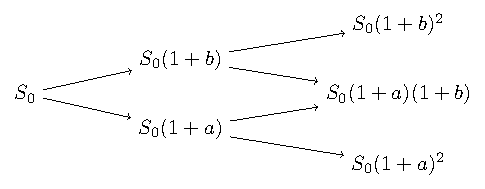
\includegraphics[width=.5\textwidth]{./stochv_abbildungen/stochv_1_2_crr}
		\captionof{figure}{Cox-Ross-Rubinstein-Modell}
		&
		$\hookrightarrow$ rekombinierender Baum, \newline
		Ereignisse $\omega$ entsprechen Pfaden im Baum
	\end{tabularx}	
\end{beispiel}

\begin{beispiel}[Black-Scholes-Modell, zeitstetig]
	Beim Black-Scholes-Modell handelt es sich um ein zeitstetiges Modell auf einem unendlichen Wahrscheinlichkeitsraum.
	\begin{equation*}
		\begin{aligned}
		S_t^0 &= e^{rt} && (\text{Verzinsung mit konstanter Rate } r) \\
		S_t^1 &= S_0^1 * \exp\brackets{(\mu-\frac{\sigma^2}{2}) + \sigma B_t} &&\mit \mu \in \R, \sigma > 0, S_0^1 > 0
		\end{aligned}
	\end{equation*}
	Der Term $\mu-\frac{\sigma^2}{2}$ beschreibt dabei eine Trendkomponenten, $B_t$ eine ''Brownsche Bewegung`` (zeitstetiger Prozess).
	\begin{center}
		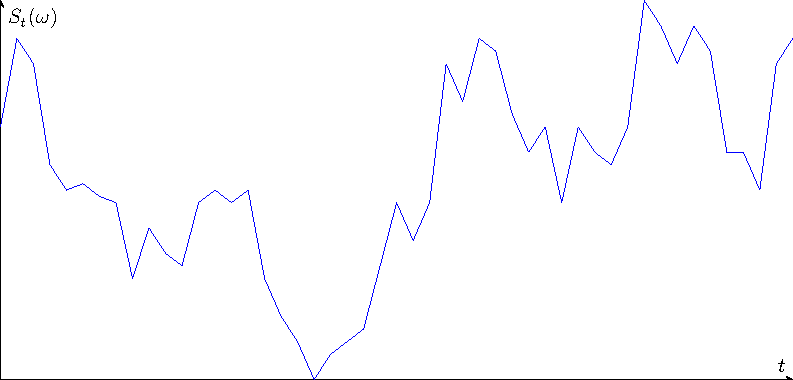
\includegraphics[width=.5\textwidth]{./stochv_abbildungen/stochv_1_2_bsm}
		\captionof{figure}{Black-Scholes-Modell}
	\end{center}
\end{beispiel}


\section{Anleihen und grundlegende Beispiele für Derivate}

Hier betrachten wir immer nur ein Basisgut $S_t = S_t^1$.

\begin{enumerate}[leftmargin=*, label=(\alph*)]
	\item \begriff{Anleihe} [bond] (genauer: Null-Kupon-Anleihe [zero-coupon bond])
	
	Der Emittent (Herausgeber) einer Anleihe mit Endfälligkeit [maturity] $T$ garantiert dem Käufer zum Zeitpunkt $T$ den Betrag $N$ (EUR/USD/...) zu zahlen.
	Typische Emittenten sind z.B. Staaten [government bond] oder Unternehmen (als Alternative zur Kreditaufnahme).
	Nach Emission werden Anleihen auf dem Sekundärmarkt weiterverkauft, d.h. liquide gehandelte Wertpapiere. 
	
	\begin{tabular}{ll}
		Preis bei Emission: & $B(0,T)$ \\
		Preis bei Weiterverkauf zum Zeitpunkt $t \le T$: & $B(t,T)$ \\
	\end{tabular}
	
	Es ist $B(T,T) = N$ und wir normieren stets $N=1 \follows B(T,T)=1$.
	
	Anleihen von West-/ Nord-/ Mitteleuropäischen Staaten und den USA sowie Kanada werden als risikolos betrachtet (sichere Zahlung). Sonst: Kreditrisiko
	
	Risikofreie Anleihen können als Numeraire $S_t^0 = B(t,T)$ genutzt werden.
	
	\begin{center}
		%TODO BILD (1)
		\includegraphics[width=.5\textwidth]{example-image}
		\captionof{figure}{Zahlungsstrom einer Anleihe}
	\end{center}
	
	\item \begriff{Terminvertrag} [forward contract]
	
	aus Käufersicht: Vereinbarung zu bestimmtem zukünftigen Zeitpunkt $T$ eine Einheit des Basisguts $S$ zum Preis $K$ zu kaufen (Kaufverpflichtung). Beliebt ist dieser bei Rohstoffen und Elektrizität.
	
	Auszahlungsprofil: $F_T = S_T - K$
	Preis zum Zeitpunkt $t$: $F_t$
	
	\begin{center}
		%TODO BILD (2)
		\includegraphics[width=.5\textwidth]{example-image}
		\captionof{figure}{Auszahlungsprofil eines Terminvertrags}
	\end{center}
	
	
	\item \begriff{(Europäische) Put- bzw. Call-Option}
	
	Recht zu einem zukünftigen Zeitpunkt $T$ eine Einheit des Basisguts $S$ zum Preis $K$ zu verkaufen (put) bzw. zu kaufen (call)
	$\to$ keine Kaufverpflichtung !
	% Vergleich zum Terminvertrag: keine Pflicht
	
	Auszahlungsprofil:
	\begin{itemize}
		\item Call: $C_T = \begin{cases} S_T - K & S_T \ge K \\ 0 & S_T < K \end{cases} = \brackets{S_T - K}_+$
		%TODO Bild (3)
		\item Put: $P_T = \begin{cases} 0 & S_T \ge K \\ K - S_T & S_T < K \end{cases} = \brackets{K - S_T}_+$ 
		%TODO Bild (4)
	\end{itemize}

	\item \begriff{Amerikanische Put- bzw. Call-Option}
	
	wie Put/Call, aber mit Ausübung zu beliebigem Zeitpunkt $\tau \in [0,T]$.
	
	\begin{tabular}{ll}
		Preis zum Zeitpunkt $t$: & $P_t^{AM}$, $C_t^{AM}$ \\
		Auszahlungsprofil zum Zeitpunkt $\tau$: & $\brackets{S_\tau - K}_+$, $\brackets{K - S_\tau}_+$
	\end{tabular}
	
	Der Zeitpunkt $\tau$ muss im Allgemeinen als Lösung eines stochastischen Optimierungsproblems bestimmt werden (optimales Stopp-Problem).
\end{enumerate}
\section{Elementare Replikations- und Ar"-bitrage"-argumente}

Was können wir (mit elementaren Mitteln) über die ''fairen`` Preise $B(t,T), F_t, C_t, P_t$ aussagen?

Wir verwenden:

\begin{itemize}[topsep=-\parskip]
	\item \begriff{Replikationsprinzip}: zwei identische, zukünftige Zahlungsströme haben auch heute denselben Wert (ein Zahlungsstrom ''repliziert`` den anderen)
	\item \begriff{No-Arbitrage-Prinzip}: ''Ohne Kapitaleinsatz kann kein sicherer Gewinn ohne Verlustrisiko erzielt werden.`` (Arbitrage = risikofreier Gewinn)
	\item \begriff{Superreplikationsprinzip} (schwächere Form des Replikationsprinzips): Ist ein Zahlungsstrom in jedem Fall größer als ein anderer, so hat er auch heute den größeren Wert.
\end{itemize}

\begin{center}
	\begin{tabular}{|c|c|c|}
		\hline
		stark & Replikationsprinzip & eingeschränkt anwendbar \\
		$\downarrow$ & Superreplikationsprinzip & $\uparrow$ \\
		schwach & No-Arbitrage-Prinzip & immer anwendbar \\
		\hline
	\end{tabular}
\end{center}

\begin{lemma} % 1.1
	Für den Preis $C_T$ des europäischen Calls gilt:
	\begin{equation*}
		\brackets{S_t - K B(t,T)}_+ \le C_t \le S_t
	\end{equation*}
\end{lemma}
\begin{proof}
	untere Schranke: Für Widerspruch nehme an, dass $S_t - K B(t,T) - C_t = \epsilon > 0$.
	
	\begin{center}
		\begin{tabular}{|l|c|cc|} % Wert in T über rechte beide Spalten
			\hline \multirow{2}{*}{Portfolio} & \multirow{2}{*}{Wert in $t$} & \multicolumn{2}{c|}{Wert in $T$} \\
			&& $S_T \le K$ & $S_T > K$ \\ \hline \hline
			Kaufe Call & $C_t$ & $0$ & $S_T - K$ \\
			Verkaufe Basisgut & $-S_T$ & $-S_T$ & $-S_T$ \\
			Kaufe Anleihe & $\epsilon + K B(t,T)$ & $\frac{\epsilon}{B(t,T)} + K$ &  $\frac{\epsilon}{B(t,T)} + K$ \\ \hline
			$\Sigma$ & $0$ & $K - S_T + \frac{\epsilon}{B(t,T)} > 0$ & $\frac{\epsilon}{B(t,T)} > 0$ \\
			& kein Anfangskapital & \multicolumn{2}{c|}{sicherer Gewinn}\\ \hline
		\end{tabular}
	\end{center}

	Dies steht jedoch im Widerspruch zum No-Arbitrage-Prinzip. Somit ist $S_t - K B(t,T) \le C_T$. Außerdem ist $C_t \ge 0$, d.h. $C_t \ge \brackets{S_t - K B(t,T)}_+$.
	
	obere Schranke: $\nearrow$ Übung
\end{proof}

\begin{lemma}[Put-Call-Parität] % 1.2
	Für Put $P_t$, Call $C_t$ mit selbem Ausübungspreis $K$ und Basisgut $S_t$ gilt
	\begin{equation*}
		C_t - P_t = S_t - B(t,T) * K
	\end{equation*}
	%TODO Bild (5)
\end{lemma}
\begin{proof}
	Mit Replikationsprinzip:
	
	\begin{center}
		\begin{tabular}{|l|c|cc|}
			\hline 
			\multirow{2}{*}{Portfolio 1} & \multirow{2}{*}{Wert in $t$} & \multicolumn{2}{c|}{Wert in $T$} \\
			&& $S_T \le K$ & $S_T > K$ \\ \hline \hline
			Kaufe Call & $C_t$ & $0$ & $S_T - K$ \\
			Kaufe Anleihe & $K * B(t,T)$ & $K$ & $K$ \\ \hline
			Wert Portfolio 1 & $C_t + K * B(t,T)$ & K & $S_T$ \\ 
			\hline
		\end{tabular}
	\end{center}

	\begin{center}
		\begin{tabular}{|l|c|cc|}
			\hline 
			\multirow{2}{*}{Portfolio 2} & \multirow{2}{*}{Wert in $t$} & \multicolumn{2}{c|}{Wert in $T$} \\
			&& $S_T \le K$ & $S_T > K$ \\ \hline \hline
			Kaufe Put & $P_t$ & $K - S_T$ & $0$ \\
			Kaufe Basisgut & $S_t$ & $S_T$ & $S_T$ \\ \hline
			Wert Portfolio 2 & $P_t + S_t$ & $K$ & $S_T$ \\ 
			\hline
		\end{tabular}
	\end{center}

	Replikationsprinzip: $C_t + K * B(t,T) = P_t + S_t \follows C_t + P_t = S_t - K*B(t,T)$
\end{proof}

\end{document}